\documentclass[11pt]{article}
\usepackage[sc]{mathpazo} %Like Palatino with extensive math support
\usepackage{fullpage}
\usepackage[round, authoryear]{natbib}
\linespread{1.7}
\usepackage[utf8]{inputenc}
\usepackage{lineno}
\usepackage{titlesec}
\usepackage{graphicx}
\usepackage{color}
\usepackage{amsmath}
\usepackage{ulem}  % for equations

\title{Supplementary Information:\\ On multiple infections by parasites with complex life cycles}

% This version of the LaTeX template was last updated on
% November 8, 2019.

%%%%%%%%%%%%%%%%%%%%%
% Authorship
%%%%%%%%%%%%%%%%%%%%%
% Please remove authorship information while your paper is under review,
% unless you wish to waive your anonymity under double-blind review. You
% will need to add this information back in to your final files after
% acceptance.

%\author{Phuong Linh Nguyen$^{1,\ast}$ \& 
%Chaitanya S. Gokhale$^{2,3}$
%}
\date{}

\begin{document}
\maketitle

\renewcommand{\theequation}{SI.\arabic{equation}}
\setcounter{equation}{0}

\renewcommand{\thefigure}{SI.\arabic{figure}}
\renewcommand{\thefigure}{SI.\arabic{figure}}
\setcounter{figure}{0}

\renewcommand{\thetable}{SI.\arabic{table}}
\setcounter{table}{0}

\section*{SI 1. Reproduction ratio $R_0$}

The reproduction ratio of the parasite is derived from the dynamical system of the parasite which only include infected intermediate and definitive hosts and the free-living parasite pool. The dynamical system can be written in matrix form as followed:
\[
\frac{d \mathbf{n}}{dt} = \mathbf{M} \mathbf{n}
\]

where $\mathbf{n}$ is the vector of singly and doubly infected intermediate hosts, singly and doubly infected definitive hosts and free-living parasites ($dI_w, I_{ww}, D_w, D_{ww}, W$) and $\mathbf{M}$ is the matrix that describes the dynamics
\[ \mathbf{M} = 
\begin{pmatrix}
- d - \alpha_w - P_w & 0 & 0 & 0 & (1 - p) \gamma I_s \\
0 & -d - \alpha_{ww} - P_{ww} & 0 & 0 & p \gamma I_s \\
h (\beta_w + \rho ) D_s &  h (\beta_{ww} + \rho) (1-q) D_s &-\lambda_w -   (1-q)\lambda_{ww}  -\mu -\sigma_w & 0 & 0 \\
0 &  h (\beta_{ww} + \rho ) q D_s  & \lambda_w +  (1-q) \lambda_{ww}  & -\mu - \sigma_{ww} & 0 \\
 0 & 0 & f_w & f_{ww} &- \delta - \gamma I_s  \\
\end{pmatrix}
\]

The matrix $\mathbf{M}$ can be written as $\mathbf{M} = \mathbf{F} - \mathbf{V}$, where

\[
\mathbf{F} = 
\begin{pmatrix}
0 & 0 & 0 & 0 & 0  \\
0 & 0 & 0 & 0 & 0  \\
0 & 0 & 0 & 0 & 0  \\
0 & 0 & 0 & 0 & 0  \\
0 & 0 & f_w & f_{ww} & 0
\end{pmatrix}
\]

is the matrix in which its elements are the reproduction contribution of one compartment to the other compartments in the next generation, and

\[
\mathbf{V} = 
\begin{pmatrix}
\alpha_w + d + P_w  & 0 & 0 & 0 & - (1 - p) \gamma  I_s\\
 0 & \alpha_{ww} + d + P_{ww} & 0 & 0 & - p \gamma I_s \\
- h(\rho + \beta_w) D_s & - h(\rho + \beta_{ww})  (1 - q) D_s & \lambda_w +  \lambda_{ww} (1-q) + \mu + \sigma_w & 0 & 0 \\
 0 & -h (\rho + \beta_{ww}) q D_s  & -\lambda_w -  \lambda_{ww} (1 - q) & \mu + \sigma_{ww} & 0 \\
 0 & 0 & 0 & 0 & \delta + \gamma I_s \\
\end{pmatrix}
\]

is the matrix in which its elements include death rates or transition rates from one compartment to the others \citep{Diekmann1990, Diekmann2009, hurford:JRSI:2010}. 

The reproduction ratio $R_0$ is then the leading eigenvalue of the matrix $\mathbf{F}.\mathbf{V}^-1$, evaluated at the disease-free equilibrium of the intermediate and definitive hosts $I_s^*$, $D_s^*$, and $I_w = I_{ww} = D_w = D_{ww} = 0$.

\section*{SI 2. Equilibrium stability - linear birth function for intermediate hosts}

The jacobian matrix of the system of equations (1), (2), and (3), as given in the main text  is evaluated at the disease-free equilibrium, and $B(D_s, D_w, D_{ww}, I_s, I_w, I_{ww}) = \rho c D_{total} I_{total}$ is

\[
\begin{pmatrix}
	0 & r & r & -\frac{\mu}{c} & -\frac{\mu }{c} & -\frac{\mu }{c} & -\frac{\gamma  \mu }{c \rho } \\
	0 & -\alpha_w + \frac{(\beta_w + \rho ) (d-r)}{\rho } - d & 0 & 0 & 0 & 0 & \frac{\gamma  \mu  (1-p)}{c \rho } \\
	0 & 0 & -\alpha_{ww} + \frac{(\beta_{ww} + \rho ) (d-r)}{\rho } - d & 0 & 0 & 0 & \frac{\gamma  \mu  p}{c \rho } \\
	-c (d-r) & \frac{\beta_w (d-r)}{\rho } - c (d-r) & \frac{\beta_{ww} (d-r)}{\rho }-c (d-r) & 0 & \mu  & \mu  & 0 \\
	0 & -\frac{\beta_w (d-r)}{\rho } & -\frac{ \beta_{ww} (1-q) (d-r)}{\rho } & 0 & -\mu - \sigma_w & 0 & 0 \\
	0 & 0 & -\frac{\beta_{ww} q (d-r)}{\rho } & 0 & 0 & -\mu - \sigma_{ww} & 0 \\
	0 & 0 & 0 & 0 & f_w & f_{ww} & -\frac{\gamma  \mu }{c \rho } - \delta  \\
\end{pmatrix}
\]

This jacobian has seven eigenvalues, two of which have explicit expressions as $\pm \sqrt{d - r}$. Here, we always have $r > d$ so that the equilibrium is positive, therefore these two eigenvalues are always pure imaginary. We cannot obtain the explicit expression of the other five eigenvalues but the dynamics remain unstable regardless of their values.

\section*{SI 3. Invasion of parasite - Linear birth function }


$R_0 > 1$ when the transmission rate from the parasite pool to intermediate hosts satisfies

\begin{align}
	\gamma > & \frac{c \delta  \rho  (\mu +\sigma_w) (\mu + \sigma_{ww}) (\beta_w (r-d)+\rho  (\alpha_w+ r)) (\beta_{ww} (r-d)+\rho  (\alpha_{ww}+r))}{\mu } \notag \times \\
	& \frac{1}{\begin{pmatrix}
			d^2 \left(f_w h (\mu  + \sigma_{ww}) (\beta_{ww} (1-p) \rho  + \beta_w \beta_{ww} (1-p q)+\beta_w p (1-q) \rho ) - \right. \\
			\left. \beta_w (\mu + \sigma_w) (\beta_{ww} (\mu +\sigma_{ww}) - f_{ww} h p q (\beta_{ww}+\rho ))\right) + \\
			d \left(f_w h (\mu +\sigma_{ww}) (- \alpha_{ww} (1-p) \rho  (\beta_w + \rho )  \right.  \\
			\left. - \alpha_w p (1 - q) \rho  (\beta_{ww}+\rho ) - 2 \beta_w \beta_{ww} r (1-p q) \right. + \\
			\left. \beta_w \rho  r (p (2 q-1)-1) + \rho  r (\beta_{ww} (p q + p-2)+\rho  (p q - 1))) \right. + \\
			\left. (\mu +\sigma_w) ((\mu +\sigma_{ww}) (\beta_{ww} \rho  (\alpha_w+r) + \beta_w \rho  (\alpha_{ww}+r) \right. + \\
			\left. 2 \beta_w \beta_{ww} r)-f_{ww} h p q (\beta_{ww}+\rho ) (\rho  (\alpha_w+r)+2 \beta_w r)) \right) + \\
			f_w h r (\mu +\sigma_{ww}) (\alpha_{ww} (1-p) \rho  (\beta_w+\rho )+\alpha_w p (1-q) \rho  (\beta_{ww}+\rho )+r (\beta_w+\rho ) (\beta_{ww}+\rho ) (1-p q)) - \\
			(\mu +\sigma_w) (\alpha_w \rho +r (\beta_w+\rho )) (\alpha_{ww} \rho  (\mu +\sigma_{ww})+r (\beta_{ww}+\rho ) (-f_{ww} h p q+\mu +\sigma_{ww}))
		\end{pmatrix}}
\end{align}

and the reproduction rates $f_w$ and $f_{ww}$ satisfies either of the following conditions

\begin{align}
	f_{ww} \geq \frac{(\mu + \sigma_{ww}) (-\alpha_{ww} \rho + \beta_{ww}d-r (\beta_{ww}+\rho ))}{h p q (\beta_{ww}+\rho ) (d-r)}
\end{align}
or

\begin{align}
	f_{ww} < &  \frac{(\mu + \sigma_{ww}) (-\alpha_{ww} \rho + \beta_{ww}d-r (\beta_{ww}+\rho ))}{h p q (\beta_{ww}+\rho ) (d-r)} \notag \\
	f_w > & \frac{(\mu + \sigma_w) (- \alpha_w \rho + \beta_w d-r (\beta_w+\rho ))}{h (d-r) (\mu + \sigma_{ww})} \times  \\
	          & \frac{(r-d) (\beta_{ww} (\mu + \sigma_{ww}) - f_{ww} h p q (\beta_{ww}+\rho ))+\rho  (\mu +\sigma_{ww}) (\alpha_{ww} + r)}{\begin{pmatrix}
	          		d (-\beta_{ww} (1-p) \rho +\beta_w \beta_{ww} (-(1-p q))-\beta_w p (1-q) \rho ) + \\
	          		\alpha_{ww} (1-p) \rho  (\beta_w+\rho )+\alpha_w p (1-q) \rho  (\beta_{ww}+\rho )+r (\beta_w+\rho ) (\beta_{ww}+\rho ) (1-p q)
	          	\end{pmatrix}}
\end{align}

\section*{SI 4. Equilibrium stability - Non-linear birth function for intermediate hosts }
The disease free equilibrium of the system of equations (1), (2), (3) given in the main text is

\begin{align}
	I_s^* & = \frac{\mu}{c \rho} \\
	D_s^* & = \frac{c \rho  (r-d)-k \mu  r}{c \rho^2}
\end{align}

$D_s^*$ is positive if $X = c \rho  (r-d)-k \mu  r$ is positive.

The eigenvalues of the Jacobian matrix established at the disease free equilibrium are roots of the following polynomial:

\begin{equation}
	A_4 \lambda^4 + A_3 \lambda^3 + A_2 \lambda^2 + A_1 \lambda + A_0
\end{equation}

The disease free equilibrium is stable if the above polynomial has all negative real roots. Using the Descarte rule, the polynomial has all negative real root if all the coefficients are positive.

We know that $A_4 = 1$ is always positive. 

\begin{equation}
	A_3 = \rho ^7 \left(X (\beta_w + \beta_{ww}+2 \rho ) + c \rho^2  (2 \alpha +\delta +\mu +\sigma + 2 d  )+\gamma  \mu  \rho \right)
\end{equation}

is always postive as all the elements of $A_3$ are positive.

\begin{align}
	A_2 = & \rho^{14} \left(c \rho ^3 (c \rho  (\alpha ^2+2 \alpha  (\delta +\mu +\sigma )+\delta  (\mu +\sigma ))+(2 \alpha +d+\mu +\sigma ) (c d \rho +\gamma  \mu )+c d \rho  (2 \delta +\mu +\sigma )+\gamma  d \mu ) \right. \notag \\
	&\left. +X (\beta_w + \beta_{ww}+2 \rho ) (c \rho ^2 (\alpha +d+\delta +\mu +\sigma )+\gamma  \mu  \rho )+X^2 (\beta_w+\rho ) (\beta_{ww}+\rho )\right)
\end{align}
is always positive because all elements of $A_2$ are positive.

\begin{align}
	A_1 =  \rho ^{22} \left(c^2 \rho ^2 A_{10} +A_{11}-c \gamma  X  A_{12} f_w h \mu  \rho ^2 \right)
\end{align}
is positive if reproduction in single infection $f_w$, the probability to sucessfully established in the definitive host $h$, and cooperation in reproduction $\epsilon$ are small enough because 
\begin{equation}
	A_{10} = \alpha  \rho ^2 (\alpha  \gamma  \mu +\alpha  c \rho  (\delta +\mu +\sigma )+2 (\mu +\sigma ) (c \delta  \rho +\gamma  \mu ))
\end{equation}
is always positive positive, and
\begin{align}
	A_{11} = & c \rho ^2 (2 c d \rho  \rho + X (\beta_w + \beta_{ww}+2 \rho )) (\alpha  \gamma  \mu +\alpha  c \rho  (\delta +\mu +\sigma ) +  (\mu +\sigma ) (c \delta  \rho +\gamma  \mu )) + \\
	& c d \rho ^2 (c \rho  (\delta +\mu +\sigma )+\gamma  \mu ) (c d \rho ^2+X (\beta_w+\beta_{ww}+2 \rho )) + \\
	& X^2 (\beta_w+\rho ) (\beta_{ww}+\rho ) (c \rho  (\delta +\mu +\sigma )+\gamma  \mu )
\end{align}
is always positive.
\begin{equation}
	A_{12} =\beta_w (1-p)+p (\beta_{ww}+q (\epsilon -1) (\beta_{ww}+\rho ))+\rho
\end{equation}
is always positive because $0 \leq p \leq 1$ and $0 \leq q \leq 1$. If $\epsilon > 1$, then $A_{12}$ is always positive. The smaller the value of $\epsilon$, the more likely $A_{12}$ is negative. However, even when $\epsilon = 0$, $A_{12} = \beta_w (1-p) + \beta_{ww} p (1-q)+\rho  (1-p q)$ is always positive.
Because $A_{12}$ is positive, if $f_w$, $h$ and $\epsilon$ are sufficiently large, $A_1$ can be negative and the polynomial will not have all negative eigenvalues.

Finally, we have

\begin{equation}
	A_0 = c^9 \rho^{31} \left(-f_w h \gamma \mu A_{00} + A_{01}\right)
\end{equation}

where 
\begin{align}
	A_{00} = X (c  \rho ^2 (\alpha +d) A_{12} + X (\beta_w+\rho ) (\beta_{ww}+\rho ) ( p q (\epsilon -1)+1))
\end{align}
is always positive, and
\begin{align}
	A_{01} = (\mu +\sigma ) (c \delta  \rho +\gamma  \mu ) (c^2 \rho ^4 (\alpha +d)^2+c X \rho ^2 (\beta_w+\rho ) (\alpha +d)+c X \rho ^2 (\beta_{ww}+\rho ) (\alpha +d)+X^2 (\beta_w+\rho ) (\beta_{ww}+\rho ))
\end{align}
is always positive. Therefore, if $f_w$ , $h$, and $\epsilon$ are sufficiently large, $A_0$ could be negative, leading to non-negative eigenvalues of the polynomial.

For all the above argument, the disease free equilibrium is positive and stable if $f_w$, $h$ and $\epsilon$ are sufficiently small, eventhough we cannot deduce the explicit expression for the condition.

\section*{SI 5. Non-linear birth function for intermediate hosts - invasion condition}

The condition for parasite invasion is $R_0 > 1$, which is satisfied when

%\begin{align}
%	f_w > & \frac{(c \delta  \rho +\gamma  \mu ) (k \mu  r (\beta_w+\rho )-c \rho  (\beta_w (-d)+\rho  (\alpha +r)+\beta_w r))}{\gamma  \mu  (c \rho  (d-r)+k \mu  r)} \notag \\
%	& \frac{(\mu +\sigma ) (k \mu  r (\beta_{ww}+\rho )-c \rho  (\beta_{ww} (-d)+\rho  (\alpha +r)+\beta_{ww} r))}{ \begin{pmatrix} c \rho  (\beta_w \beta_{ww} (d-r) (p q (\epsilon -2)+p+1) + & \\ 
%			\rho  (\alpha +r) (\beta_w (p-1)-\beta_{ww} p (q (\epsilon -2)+2))) + & \\
%			 k \mu  r (\beta_w (\beta_{ww} (p q (\epsilon -2)+p+1)-p \rho + & \\
%			 \rho )+\beta_{ww} p \rho  (q (\epsilon -2)+2)) \end{pmatrix}}
%\end{align}

\begin{align}
	f_w > \frac{\begin{pmatrix}
			(\mu +\sigma ) (c \delta  \rho +\gamma  \mu ) (k \mu  r (\beta_w+\rho )-c \rho  (\beta_w (-d)+\rho  (\alpha +r)+\beta_w r)) (k \mu  r (\beta_{ww}+\rho )- \\
			c \rho  (\beta_{ww} (-d)+\rho  (\alpha +r)+\beta_{ww} r))
		\end{pmatrix}}{\begin{pmatrix}
		\gamma  h \mu  (c \rho  (d-r)+k \mu  r) (k \mu  r (\beta_w+\rho ) (\beta_{ww}+\rho ) (p q (\epsilon -1)+1) - \\ 
		c \rho  (\beta_{ww} d (p-1) \rho -\beta_w d (\beta_{ww} + \beta_{ww} p q (\epsilon -1) + \\
		p \rho  (q (\epsilon -1)+1))+\alpha  \rho  (\beta_w+\beta_w (-p)+ \\ 
		p (\beta_{ww}+\beta_{ww} q (\epsilon -1)+q \rho  (\epsilon -1))+\rho )+r (\beta_w+\rho ) (\beta_{ww}+\rho ) (p q (\epsilon -1)+1))
	\end{pmatrix}}
\end{align}

\section*{Tables}


\begin{table}[!ht]
\caption{Description of variables and parameters}
\label{table:varpardescription}
\centering
\begin{tabular}{c|p{10cm}}%{|p{2.5cm}|p{12cm}|} 
\hline
Parameters and Variables    &  Description  \\
\hline
$I_i$  & Density of intermediate hosts that are susceptible $i=s$, singly infected $i=w$, or doubly infected $i=ww$ \\
\hline
$D_i$ & Density of definitive hosts that are susceptible $i=s$, singly infected $i=w$, or doubly infected $i=ww$ \\
\hline
$W$ & Density of parasites released from definitive hosts into the environment \\
\hline
$d$ & Natural death rate of intermediate hosts \\
\hline
$\alpha_i$ & Additional death rate of intermediate hosts due to infection by a single parasite ($i = w$) or two parasites ($i = ww$) \\
\hline
$p$ & Probability that two parasites cotransmit from the environment to an intermediate host \\
\hline
$\gamma$ & Transmission rate of parasites in the environment to intermediate hosts \\
\hline
$\mu$ & Natural death rate of definitive hosts \\
\hline
$\sigma_i$ & Additional death rate of definitive hosts due to infection by a single parasite ($i = w$) or two parasites ($i = ww$) \\
\hline
$\sigma_i$ & Additional death rate of the hosts due to being infected by a singly parasite ($i = w$) or two parasites ($i = ww$) \\
\hline
$q$ & Probability that two parasites cotransmit from intermediate hosts to definitive hosts \\
\hline
$\beta_i$ & Transmission rate of parasites from intermediate hosts to definitive hosts \\
\hline
$f_i$ & Reproduction rate of parasites in singly infected definitive hosts ($i = w$) or doubly infected hosts ($i = ww$)\\
\hline
$\delta$ & Natural death rate of parasites in the environment \\
\hline 
$h$ & Probability that the parasites successfully established inside the definitive host 
\end{tabular}
\bigskip{}
\end{table}

\section*{Supplementary Figure}
%
\begin{figure}[!ht]
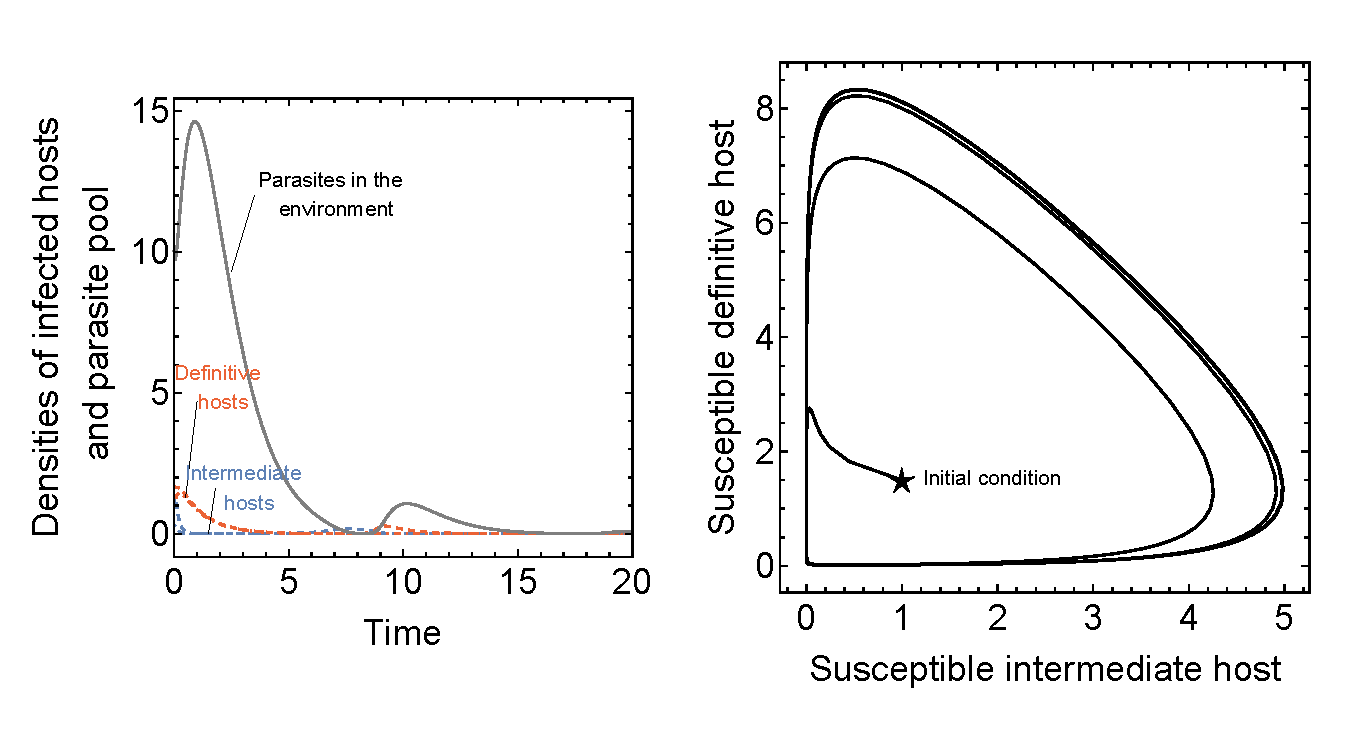
\includegraphics[width=\textwidth]{Figures/diseasefree_linear.pdf}
\caption{Disease-free equilibrium using linear birth function, where parasite goes extinct (left panel), and susceptible hosts demonstrate cyclic dynamics (right panel). Solid gray line indicate the density of free-living parasites, blue lines indicate infected intermediate hosts while red lines indicate infected definitive hosts. Dashed lines indicate singly infected hosts while dot-dashed lines indicate doubly infected hosts. Parameter values  $\rho = 1.2, \  d = 0.9, \  r = 2.5, \ \gamma = 2.9, \ \alpha_w =  \alpha_{ww} =  0, \ \beta_w  = 1.5, \ \beta_{ww} = 1.5, \ p = 0.1,  \ c = 1.4, \ \mu = 0.9,  \ \sigma_w = \sigma_{ww} = 0, \ q = 0.01, \  f_w = 6.5, \  f_{ww} = 7.5, \ \delta = 0.9$,$h_1 = h_2 = 0.8$, $R_0 = 4.997$ } 
\label{fig:diseasefree:linear}
\end{figure}

\bibliographystyle{evolution}
\bibliography{references}

\end{document}